\documentclass[aspectratio=169,11pt,t]{beamer}
% ============================================================
%  ksa-cs-v2: ksa-cs-lecture-template.tex 스타일 + 한글, v2 덱(16:9)용.
%    - 짙은 네이비 헤드라인 (섹션 이름 + 프레임마다 점)
%    - 꽉 찬 파란 제목 막대, 둥근 그림자 블록
%    - 한글: Noto Sans CJK KR (fontspec)
%  사용:
%    \documentclass[aspectratio=169,11pt,t]{beamer}
%    \input{<..>/theme/ksa-cs-v2.tex}
%  ksa-theme.tex 의 매크로(\kb \kq, ksablue/ksared 등)도 같은 이름으로 둔다
%  -> v2 덱 본문을 거의 그대로 옮길 수 있다.
% ============================================================

\usepackage{fontspec}
\usepackage{amsmath,amssymb}
\usepackage{tikz}
\usepackage{listings}
\usepackage{graphicx}
\usepackage{booktabs}
\usepackage{varwidth}
% enumitem 은 넣지 않는다 (beamer 글머리표가 사라진다)

\defaultfontfeatures{Ligatures=TeX}
\setmainfont{Noto Sans CJK KR}
\setsansfont{Noto Sans CJK KR}
\setmonofont{Noto Sans Mono CJK KR}[Scale=0.92]
\usefonttheme{professionalfonts}

% ---------- 기본 틀 ----------
\usetheme{default}
\useinnertheme[shadow=true]{rounded}
\setbeamertemplate{navigation symbols}{}
\setbeamersize{text margin left=1em,text margin right=1em}

% ---------- 색 (템플릿 원본 값) ----------
\definecolor{navydark}{HTML}{191959}
\definecolor{navydim}{HTML}{8888B0}
\definecolor{navytitle}{HTML}{262686}
\definecolor{navyblue}{HTML}{3333B2}
\definecolor{blockbodybg}{HTML}{E9E9F3}
\definecolor{examplegreen}{HTML}{006000}
\definecolor{examplebg}{HTML}{E5EFE5}
\definecolor{alertred}{HTML}{BF0000}
\definecolor{alertbg}{HTML}{F9E5E5}
% ksa-theme.tex 와 같은 이름 (본문 호환)
\colorlet{ksablue}{navytitle}
\colorlet{ksabluedk}{navydark}
\definecolor{ksagold}{HTML}{D6CBB1}
\definecolor{ksagolddk}{HTML}{A9976B}
\colorlet{ksared}{alertred}
\definecolor{ksagray}{HTML}{5B5B5B}

\setbeamercolor{structure}{fg=navyblue}
\setbeamercolor{alerted text}{fg=alertred}
\setbeamercolor{frametitle}{bg=navytitle,fg=white}
\setbeamercolor{title}{fg=white,bg=navytitle}
\setbeamercolor{block title}{bg=navytitle,fg=white}
\setbeamercolor{block body}{bg=blockbodybg,fg=black}
\setbeamercolor{block title example}{bg=examplegreen,fg=white}
\setbeamercolor{block body example}{bg=examplebg,fg=black}
\setbeamercolor{block title alerted}{bg=alertred,fg=white}
\setbeamercolor{block body alerted}{bg=alertbg,fg=black}
\setbeamercolor{item}{fg=navyblue}
\setbeamertemplate{itemize item}[circle]
\setbeamertemplate{itemize subitem}[triangle]

% ---------- 헤드라인: miniframes (섹션 이름 + 점) ----------
\useoutertheme[subsection=false]{miniframes}
\setbeamerfont{section in head/foot}{size=\tiny}
\setbeamercolor{section in head/foot}{bg=navydark,fg=white}
\setbeamercolor{mini frame}{fg=white}
\setbeamertemplate{mini frames}[circle]

% ---------- 제목 막대: 폭 꽉 채움, 두 줄까지 ----------
\setbeamerfont{frametitle}{size=\normalsize,series=\bfseries}
\setbeamertemplate{frametitle}{%
  \nointerlineskip
  \begin{beamercolorbox}[wd=\paperwidth,ht=2.7ex,dp=1.1ex,leftskip=.3cm,rightskip=.3cm]{frametitle}%
    \usebeamerfont{frametitle}\insertframetitle
  \end{beamercolorbox}}

% ---------- 쪽 번호: 오른쪽 아래 ----------
\setbeamertemplate{footline}{%
  \hfill
  {\color{navydim}\scriptsize\insertframenumber\,/\,\inserttotalframenumber}%
  \hspace{3mm}\vspace{2mm}%
}

% ---------- 표지: 템플릿처럼 헤드라인은 그대로, 가운데 둥근 그림자 상자에 제목 한 줄 ----------
% 덱에서:  {\setbeamertemplate{footline}{}\begin{frame}[c,noframenumbering]\titlepage\end{frame}}
\setbeamercolor{title}{fg=white,bg=navyblue}
\makeatletter
\setbeamertemplate{title page}{%
  \vfill
  \centering
  \begin{minipage}{0.84\paperwidth}
  \begin{beamercolorbox}[wd=\linewidth,sep=7pt,center,rounded=true,shadow=true]{title}
    {\usebeamerfont{title}\inserttitle\par}%
    \ifx\insertsubtitle\@empty\else\vskip0.4em{\usebeamerfont{subtitle}\insertsubtitle\par}\fi
  \end{beamercolorbox}
  \end{minipage}\par\vskip1.6em
  {\usebeamerfont{author}\color{navytitle}\insertauthor\par}\ifx\beamer@date\@empty\vskip0.3em\else\vskip1.3em\fi
  {\usebeamerfont{institute}\color{ksagray}\insertinstitute\par}%
  \ifx\beamer@date\@empty\else\vskip0.3em{\usebeamerfont{date}\color{ksagray}\insertdate\par}\fi
  \vfill
}
\makeatother
\setbeamerfont{title}{series=\bfseries,size=\Large}
\setbeamerfont{subtitle}{size=\normalsize}
\setbeamerfont{author}{size=\normalsize}
\setbeamerfont{institute}{size=\small}
\setbeamerfont{date}{size=\small}

% ksa-theme 호환: 덱이 \renewcommand{\ksacredit}{..} 를 해도 되게 (꼬리말에는 안 쓴다)
\newcommand{\ksacredit}{}

% ---------- 강조 ----------
\newcommand{\hl}[1]{\textcolor{alertred}{#1}}
\newcommand{\hlb}[1]{\textcolor{navyblue}{#1}}
\newcommand{\kb}[1]{\textbf{\color{ksablue}#1}}
\newcommand{\kq}[1]{\textbf{\color{ksared}#1}}

% ---------- 파이썬 코드 (템플릿과 같은 색) ----------
\definecolor{codekw}{HTML}{0033B3}
\definecolor{codebuiltin}{HTML}{BF0000}
\definecolor{codestr}{HTML}{067D17}
\definecolor{codecomment}{HTML}{8C8C8C}
\definecolor{codenum}{HTML}{1750EB}
\lstdefinestyle{py}{
  language=Python, basicstyle=\ttfamily\scriptsize,
  keywordstyle=\color{codekw}\bfseries, stringstyle=\color{codestr},
  commentstyle=\color{codecomment}\itshape, numberstyle=\color{codenum},
  emph={print,len,range,sum,input,int,str,float,list,dict,append,remove,sorted,abs,min,max},
  emphstyle=\color{codebuiltin}, showstringspaces=false, keepspaces=true,
  columns=fixed, basewidth=0.52em, aboveskip=1mm, belowskip=1mm, xleftmargin=2mm,
  breaklines=true
}
\lstset{style=py}

\usepackage{fontawesome5}
\newcommand{\paperlink}[1]{\href{#1}{\textcolor{ksablue}{\faLink}}}
% GLM 차시 (2026-11-27): 앤드류 응 CS229 강의 노트 Part III (Generalized Linear Models) 을 덱 스타일로.
% 숫자는 data.py (assert), 그림은 make_figs.py.
\setbeamerfont{author}{size=\normalsize}
\setbeamerfont{institute}{size=\small}
\graphicspath{{figs/}{../../../assets/}}
\usetikzlibrary{positioning,arrows.meta,calc}

\renewcommand{\ksacredit}{Machine Learning and Deep Learning \,\textperiodcentered\, GLM}
\title{일반화 선형 모델 (GLM)}
\subtitle{선형회귀 · 로지스틱회귀 · 소프트맥스는 한 가족}
\author{Machine Learning and Deep Learning}
\institute{KSA 2027-Spring}
\date{Sumin Han (suminhan@ksa.hs.kr)}
\begin{document}
{\setbeamertemplate{footline}{}\begin{frame}[c,noframenumbering]\titlepage\end{frame}}

\section{질문}
% --- 오늘의 질문: 기울기가 왜 같나
\begin{frame}{오늘의 질문: 왜 기울기 식이 똑같을까?}
\vfill
\centering
\renewcommand{\arraystretch}{1.35}
{\large\begin{tabular}{r|c|c|c}
 & 예측 $\hat y$ & 손실 & 기울기 $\partial J / \partial w_1$\\ \hline
선형회귀 & $z$ & \kq{오차 제곱} & $(\hat y - y)\,x$\\[-0.5em]
 & & {\small (Squared Error)} & \\
로지스틱회귀 & $\sigma(z)$ & \kq{교차 엔트로피} & $(\hat y - y)\,x$\\[-0.5em]
 & & {\small (Cross Entropy)} &
\end{tabular}}\\[0.5em]
{\large $z = w_0 + w_1 x$ \quad 손실은 다른데}\\[0.3em]
{\large 그런데 미분하면 \kb{똑같은 모양} \;$\to$\; 우연일까?}\\[0.5em]
\fcolorbox{ksablue}{ksablue!6}{\parbox{0.9\linewidth}{\centering
\textbf{오늘의 목표} \quad $y$ 의 분포 하나만 고르면 \kb{예측 함수}와 \kb{손실}이 저절로 정해진다\\[0.15em]
$\to$ 개수 같은 새 $y$ 에도 모델을 만들고, 신경망의 \kb{마지막 층 · 손실}을 고르는 근거가 된다}}
\vfill
\note{선형회귀와 로지스틱회귀를 나란히 놓아 봅시다. 둘 다 직선 z, w0 더하기 w1 x를 계산합니다. 선형회귀는 z를 그대로 예측으로 쓰고, 로지스틱회귀는 시그모이드를 씌웁니다. 손실도 다릅니다. 선형회귀는 오차 제곱, 로지스틱회귀는 교차 엔트로피입니다. 그런데 손실을 w로 미분하면, 둘 다 오차 와이햇 빼기 y에 입력 x를 곱한 똑같은 모양이 나왔습니다. 로지스틱회귀 시간에 계산으로 확인했죠. 이게 우연일까요? 오늘은 이 두 모델이 사실 한 가족이라서 그렇다는 것을 봅니다. 그 가족의 이름이 일반화 선형 모델, GLM입니다. 오늘의 목표는 아래 상자입니다. y가 어떤 분포를 따르는지 하나만 고르면, 예측 함수와 손실이 저절로 정해진다는 것을 봅니다. 그러면 오늘 볼 월드컵 골 수 같은 새로운 y에도 모델을 바로 만들 수 있고, 나중에 신경망을 만들 때 마지막 층과 손실을 왜 그렇게 고르는지 근거가 됩니다.}
\end{frame}

% --- 맞힐 값의 종류
\begin{frame}{맞힐 값 $y$ 의 종류가 다르다}
\vfill
\centering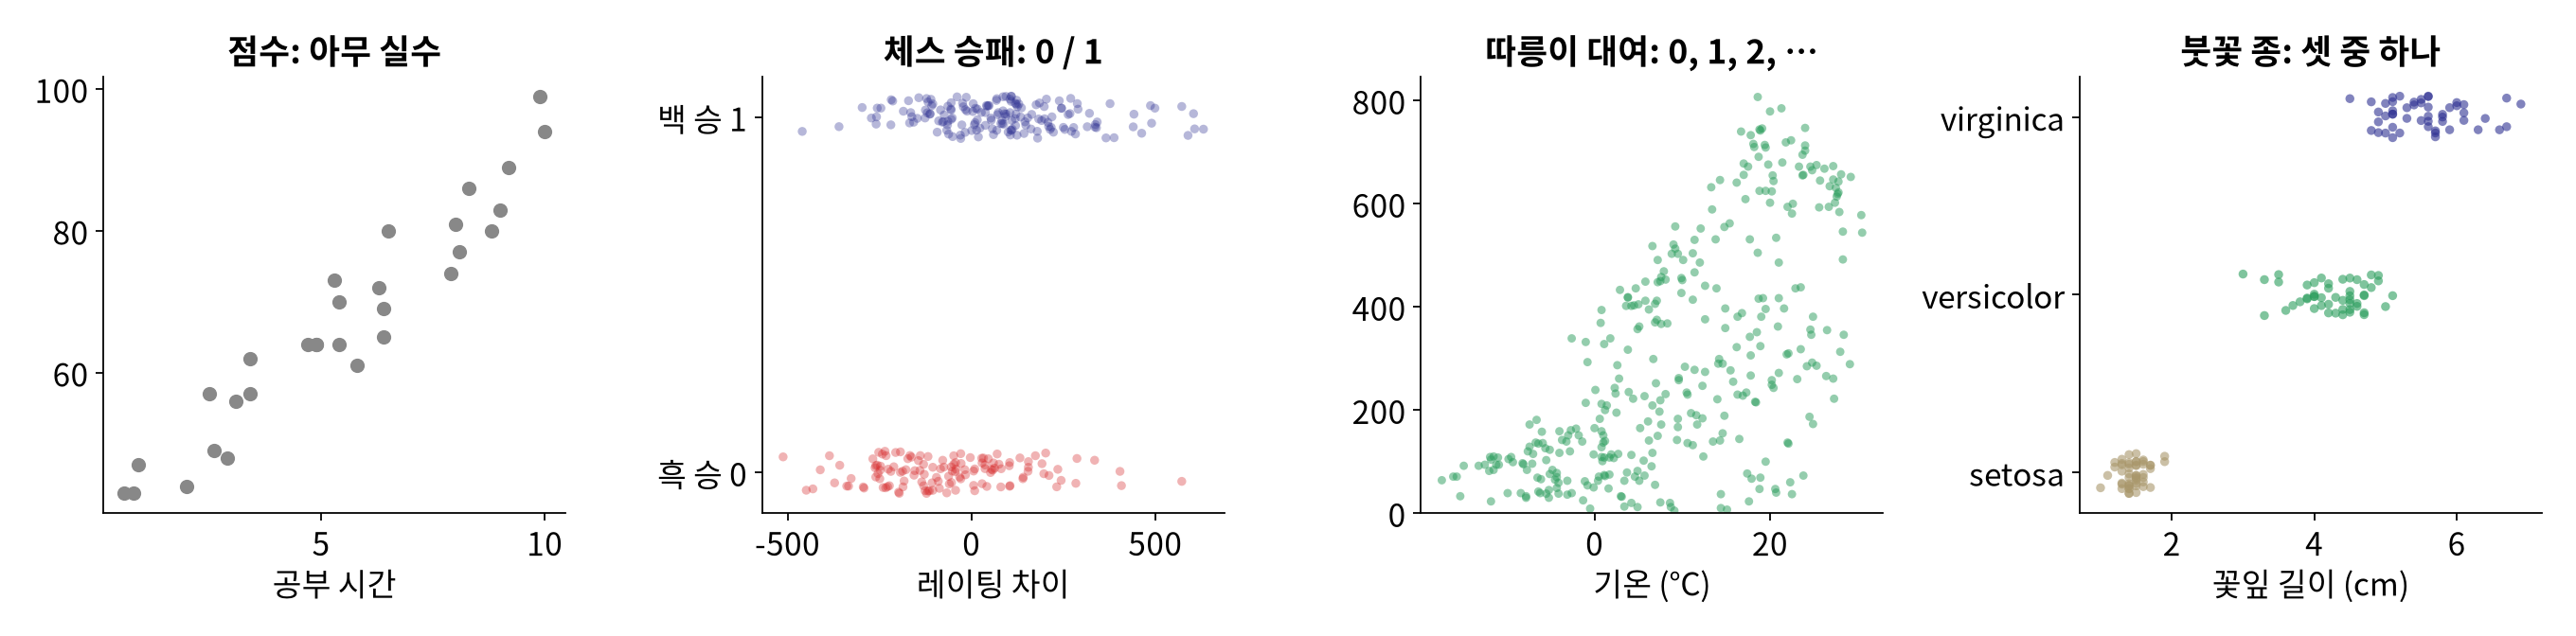
\includegraphics[width=\linewidth]{glm_types.png}\par\vskip0.3em
{\large 실수 \;·\; 0 / 1 \;·\; \kb{개수} (0 이상 정수) \;·\; \kb{셋 중 하나} \quad $\to$ 예측도 그 모양이어야 한다}\\[0.2em]
{\small 월드컵 = 본선 1930$\sim$2026, 23개 대회 1068경기 (팀마다 한 줄, 2136줄) \quad 붓꽃 = Fisher (1936) 150송이}
\vfill
\note{우리가 맞히려는 값 y는 종류가 여러 가지입니다. 1주차의 시험 점수는 아무 실수나 될 수 있습니다. 지난 시간의 체스 승패는 0 아니면 1입니다. 오늘 새로 볼 월드컵 골 수는 0, 1, 2처럼 0 이상의 정수, 개수입니다. 1930년 첫 대회부터 올해 2026년 대회까지 23개 대회 1068경기에서, 팀마다 한 경기에 넣은 골을 한 줄로 적어 2136줄입니다. 가로축은 두 팀의 실력 차이, Elo 점수 차이입니다. Elo는 체스 레이팅과 같은 방식으로, 국가대표 경기 결과로 매긴 점수입니다. 붓꽃은 꽃잎 길이로 세 종 중 하나를 맞히는 문제입니다. 예측도 y의 모양에 맞아야 합니다. 확률은 0과 1 사이, 개수는 0 이상, 세 종의 확률은 더해서 1이어야 하죠.}
\end{frame}

% --- 분포 네 개
\begin{frame}{데이터마다 맞는 분포가 있다}
\vfill
\centering
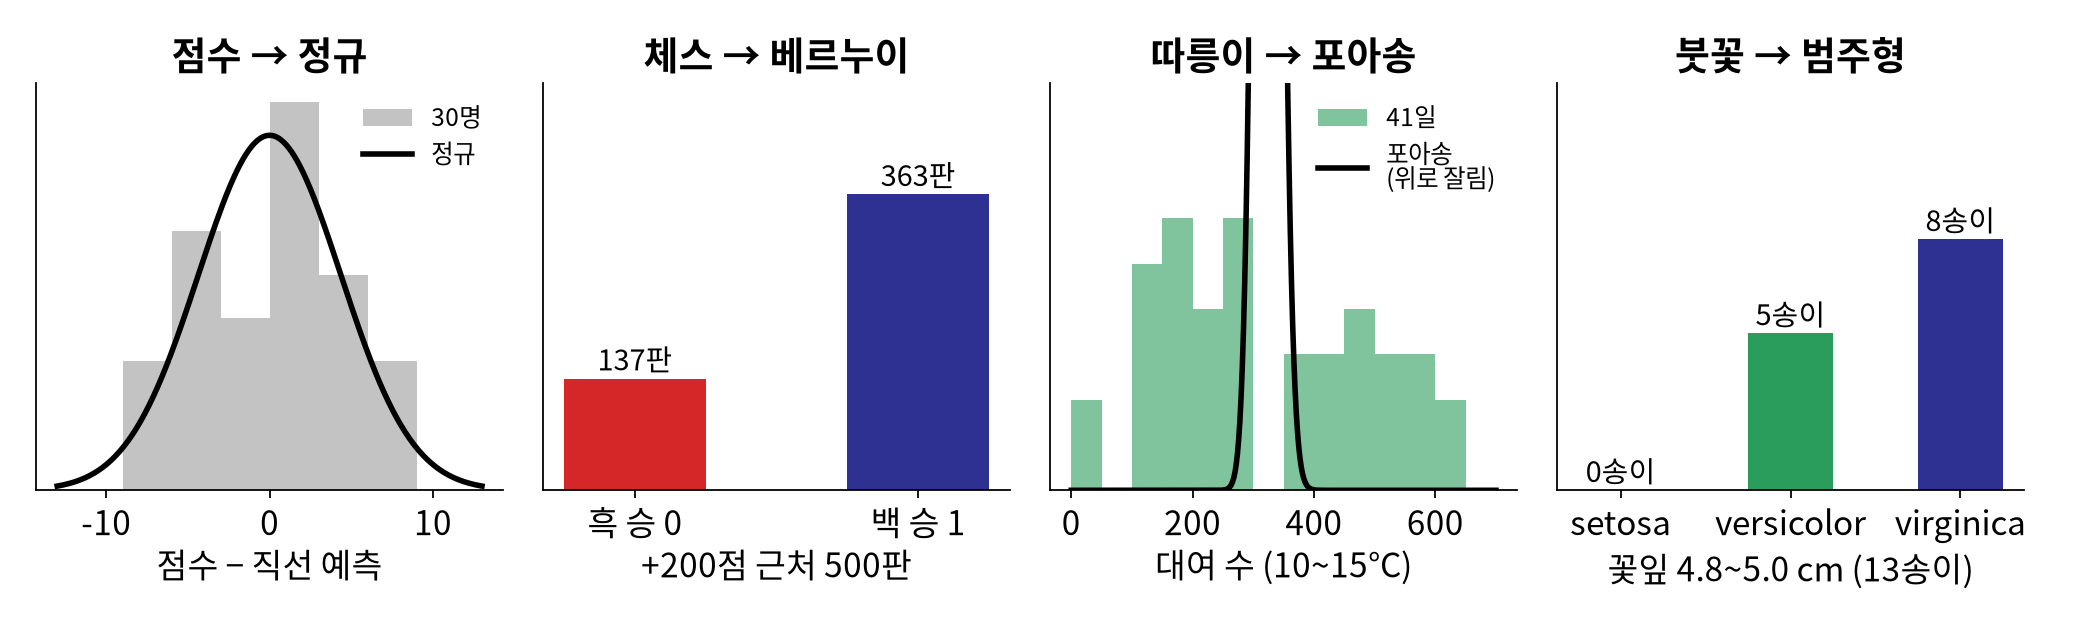
\includegraphics[width=0.95\linewidth]{glm_dists}\\[0.1em]
\renewcommand{\arraystretch}{1.2}
{\large\begin{tabular}{cccc}
\makebox[0.21\linewidth]{$\frac{1}{\sqrt{2\pi}\sigma}\,e^{-(y-\mu)^2/2\sigma^2}$} &
\makebox[0.21\linewidth]{$\phi^{\,y}(1-\phi)^{1-y}$} &
\makebox[0.21\linewidth]{$\lambda^{y}e^{-\lambda}/\,y!$} &
\makebox[0.21\linewidth]{$p(y = k) = \phi_k$}\\
$\sigma = 4.4$ 점 & $\phi = 363/500 = 0.73$ & $\lambda = 1.30$ 골 & $\phi = (0,\ 0.38,\ 0.62)$
\end{tabular}}\\[0.4em]
{\small 막대 $=$ 실제 데이터, 검은 선 $=$ 같은 평균의 분포 }
\vfill
\note{지금까지 선형회귀는 y가 정규분포를, 로지스틱회귀는 y가 베르누이 분포를 따른다고 보았습니다. 앞에서 본 네 데이터에 분포를 맞춰 봅시다. 막대가 실제 데이터, 검은 선이 같은 평균을 가진 분포입니다. 점수는 직선 예측에서 벗어난 정도를 30명 모아 보면 종 모양, 정규분포입니다. 표준편차는 4.4점입니다. 체스는 레이팅이 200점 앞선 근처 500판을 모으면 백이 363판 이겼습니다. 1일 확률 파이가 0.73인 베르누이입니다. 월드컵은 실력이 비슷한 경기, Elo 차이가 50점 안인 462줄의 골 수입니다. 평균 1.30골인 포아송과 거의 겹칩니다. 붓꽃은 꽃잎 길이 4.8에서 5.0센티미터인 13송이를 모으면 setosa 0, versicolor 5, virginica 8송이, 범주형 분포입니다. 이 네 분포의 식은 달라 보이지만, 정리하면 모두 같은 꼴이 됩니다. 다음 쪽에서 봅니다.}
\end{frame}

\section{지수족}
% --- 지수족
\begin{frame}{네 분포가 같은 꼴로 써진다: 지수족}
\vfill
\centering
{\Large\[ p(y;z) = b(y)\,\exp\!\big(\,\underbrace{z}_{\text{natural parameter}}\, \underbrace{T(y)}_{\text{sufficient statistic}} \;-\; \underbrace{a(z)}_{\text{log partition}}\,\big) \]}\vskip0.5em
{\large 정규 · 베르누이 · 포아송 · 범주형 분포가 모두 이 꼴 $=$ \kb{지수족} (exponential family)}\\[0.4em]
{\large $T, a, b$ 를 정하면 \kb{한 가족} \;·\; $z$ 를 바꾸면 그 가족 안의 분포들}\\[0.3em]
{\large $e^{-a(z)}$: 확률의 합이 1 이 되게 맞추는 몫 \quad 오늘 분포는 $T(y) = y$ (범주형만 벡터)}
\vfill
\note{앞 쪽의 네 식을 정리하면 모두 이 꼴로 쓸 수 있습니다. b of y 곱하기 exp z 곱하기 T of y 빼기 a of z. 이 꼴로 쓸 수 있는 분포들을 지수족이라고 부릅니다. z를 자연 매개변수, T of y를 충분 통계량, a of z를 로그 분배 함수라고 부릅니다. 이름은 어렵지만 역할은 간단합니다. T, a, b 세 가지를 정하면 분포의 가족 하나가 정해지고, 그 안에서 z를 바꾸면 평균이 다른 분포들이 나옵니다. 예를 들어 베르누이 가족에서 z를 바꾸면 앞면 확률이 다른 동전들이 나옵니다. e의 마이너스 a of z는 확률을 다 더했을 때 1이 되도록 맞추는 몫입니다. 오늘 보는 분포는 범주형만 빼고 T of y가 y 그대로입니다. 이제 베르누이와 정규분포를 이 꼴로 바꿔 봅시다.}
\end{frame}

% --- 베르누이 → 지수족
\begin{frame}{베르누이를 지수족 꼴로}
\vfill
\centering
{\large\begin{align*}
p(y;\phi) &= \phi^{\,y}\,(1-\phi)^{1-y} && y = 1 \text{ 이면 } \phi,\; 0 \text{ 이면 } 1-\phi\\[0.3em]
&= \exp\!\big(\,y\log\phi + (1-y)\log(1-\phi)\,\big) && \exp(\log\,\cdot\,)\\[0.3em]
&= \exp\!\Big(\,\textcolor{ksared}{\log\frac{\phi}{1-\phi}}\; y + \log(1-\phi)\,\Big) && y \text{ 로 묶기}
\end{align*}}\vskip0.6em
{\Large $z = \textcolor{ksared}{\log\dfrac{\phi}{1-\phi}}$ \;= \kb{로그 오즈}} \quad {\large $T(y) = y$, \; $a(z) = -\log(1-\phi) = \log(1 + e^{z})$, \; $b(y) = 1$}\\[0.5em]
{\large $z$ 를 $\phi$ 에 대해 풀면 \;$\phi = \dfrac{1}{1 + e^{-z}}$ \;$=$\; \kb{시그모이드!}}
\vfill
\note{베르누이는 y가 1일 확률이 파이, 0일 확률이 1 빼기 파이인 분포입니다. 이걸 한 줄로 쓰면 파이의 y제곱 곱하기 1 빼기 파이의 1 빼기 y제곱입니다. y에 1을 넣으면 파이, 0을 넣으면 1 빼기 파이가 나오죠. 둘째 줄은 exp log를 씌운 것뿐입니다. 셋째 줄은 y가 붙은 항끼리 묶었습니다. y log 파이 빼기 y log 1 빼기 파이는 y 곱하기 log 파이 나누기 1 빼기 파이입니다. 그러면 지수족의 꼴, z 곱하기 y 더하기 나머지가 됩니다. z 자리에 온 것이 빨간 부분, log 파이 나누기 1 빼기 파이입니다. 로지스틱회귀에서 본 오즈, 이길 확률 나누기 질 확률에 로그를 씌운 로그 오즈입니다. 나머지는 T of y가 y, a of z가 마이너스 log 1 빼기 파이, 파이를 z로 바꾸면 log 1 더하기 e의 z, b of y는 1입니다. 그리고 재미있는 것이 있습니다. z 이퀄 로그 오즈를 파이에 대해 풀면, 양변에 exp를 씌워 e의 z가 파이 나누기 1 빼기 파이, 정리하면 파이는 1 나누기 1 더하기 e의 마이너스 z. 바로 시그모이드입니다. 이건 조금 뒤에 로지스틱회귀를 유도할 때 다시 나옵니다.}
\end{frame}

% --- 정규 → 선형회귀
\begin{frame}{정규분포를 지수족 꼴로}
\vfill
\centering
{\Large\begin{align*}
p(y;\mu) &= \tfrac{1}{\sqrt{2\pi}}\exp\!\big(-\tfrac12 (y-\mu)^2\big) && \sigma = 1 \text{ 로 둔다}\\[0.3em]
&= \underbrace{\tfrac{1}{\sqrt{2\pi}}e^{-y^2/2}}_{b(y)}\;\exp\!\big(\,\textcolor{ksared}{\mu}\,y - \tfrac12\mu^2\,\big) && \text{제곱 전개}
\end{align*}}\vskip0.5em
{\Large $z = \textcolor{ksared}{\mu}$} \quad {\large $T(y) = y$, \; $a(z) = \tfrac12\mu^2 = \tfrac12 z^2$, \; $b(y) = \tfrac{1}{\sqrt{2\pi}}e^{-y^2/2}$}\\[0.6em]
{\small $\sigma$ 는 답 $w$ 에 영향이 없다 (1주차: 오차 제곱 최소는 $\sigma$ 와 무관)}
\vfill
\note{정규분포도 해 봅시다. 평균이 뮤인 정규분포는 1 나누기 루트 2파이 곱하기 exp 마이너스 2분의 1 y 빼기 뮤의 제곱입니다. 표준편차 시그마는 1로 둡니다. 시그마를 얼마로 두든 오차 제곱을 최소로 하는 w는 같아서 답에 영향이 없습니다. 제곱을 전개하면 y제곱 항, 뮤 y 항, 뮤제곱 항이 나옵니다. y제곱 항은 z와 상관없으니 b of y로 빼고, 남은 것이 exp 뮤 y 빼기 2분의 1 뮤제곱입니다. 지수족의 꼴과 비교하면 z가 뮤 그대로, a of z는 2분의 1 z제곱입니다. 이걸로 선형회귀가 어떻게 나오는지는 조금 뒤에 봅니다.}
\end{frame}

% --- 다른 지수족
\begin{frame}{지수족은 더 많다}
\vfill
\centering
\renewcommand{\arraystretch}{1.55}
{\large\begin{tabular}{l|l|l}
분포 & $y$ & 예\\ \hline
정규 & 실수 & 점수, 키\\
베르누이 & 0 / 1 & 승패, 스팸\\
포아송 & 개수 $0, 1, 2, \dots$ & 골 수, 시간당 손님 수\\
범주형 (multinomial) & $K$ 개 중 하나 & 붓꽃 종, 숫자 0$\sim$9\\
감마 · 지수 & 0 이상 실수 & 기다리는 시간, 수리 시간\\
베타 · 디리클레 & 확률 (0$\sim$1) & 클릭률, 비율
\end{tabular}}\\[0.8em]
{\large 다음: 이 중 \kb{아무거나} 골라서 모델을 만드는 요리법 $=$ \kb{GLM}}
\vfill
\note{정규와 베르누이 말고도 지수족은 많습니다. 개수에는 포아송, 여러 클래스 중 하나에는 범주형, 다른 이름으로 다항 분포를 씁니다. 기다리는 시간이나 수리 시간처럼 0 이상의 실수에는 감마 분포와 지수 분포, 클릭률처럼 그 자체가 확률인 값에는 베타 분포와 디리클레 분포가 있습니다. 모두 지수족 꼴로 쓸 수 있습니다. 다음은 이 중 아무 분포나 골라서, x로 y를 맞히는 모델을 만드는 요리법입니다. 그게 GLM입니다.}
\end{frame}

\section{GLM}
% --- 개수에 직선
\begin{frame}{개수를 맞히고 싶다: 직선을 그으면}
\vfill
\centering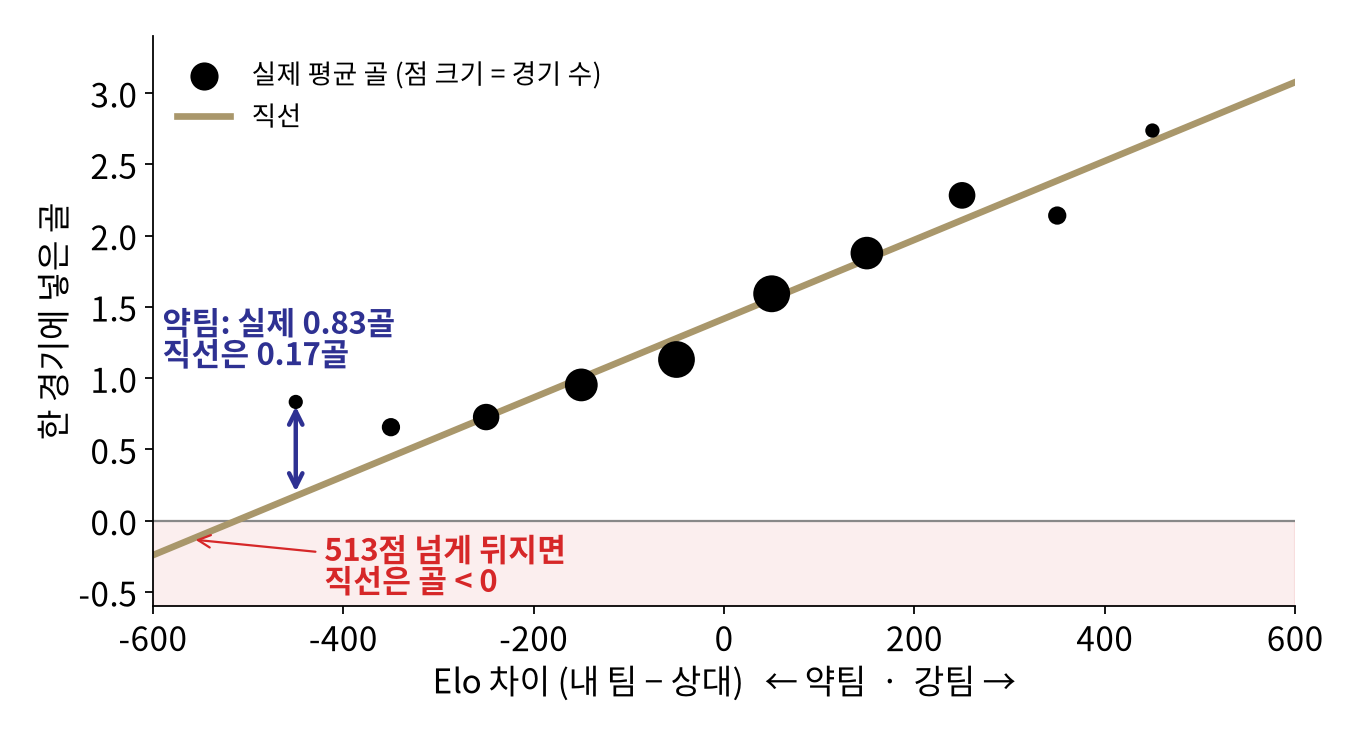
\includegraphics[width=0.56\linewidth]{glm_goals_line.png}\par\vskip0.2em
{\large 직선: 골 $= 1.418 + 0.00276 \times$ Elo 차이 \quad $\to$ \kq{513점 넘게 뒤지면 음수}}\\[0.2em]
{\large 400$\sim$500점 뒤진 약팀: 실제 \kb{0.83골}, 직선은 0.17골 \;$\to$\; 실제 평균은 직선이 아니라 \kb{휜다}}
\vfill
\note{이제 모델을 만들어 봅시다. 강의 노트는 가게에 한 시간 동안 오는 손님 수를 예로 듭니다. 우리는 월드컵에서 한 팀이 넣는 골 수를 맞혀 봅니다. 둘 다 개수입니다. 먼저 1주차처럼 직선을 그어 봅시다. 가로축은 두 팀의 Elo 차이, 왼쪽이 약팀, 오른쪽이 강팀입니다. 검은 점은 Elo 차이 100점 구간마다 실제로 한 경기에 넣은 평균 골이고, 점이 클수록 경기가 많습니다. 직선은 넣은 골이 1.418 더하기 0.00276 곱하기 Elo 차이라고 봅니다. 문제가 두 가지 보입니다. 첫째, Elo가 513점 넘게 뒤지면 직선은 음수 골을 예측합니다. 골을 마이너스로 넣을 수는 없죠. 둘째, 음수까지 가지 않아도 약팀 쪽이 틀립니다. 400점에서 500점 뒤진 약팀 18경기는 실제로 평균 0.83골을 넣었는데, 직선은 0.17골로 너무 낮게 봅니다. 검은 점들은 직선이 아니라 아래쪽이 휜 곡선을 따릅니다. 로지스틱회귀 때 0과 1을 넘는 직선 대신 시그모이드를 썼듯이, 여기도 다른 함수가 필요합니다. 포아송은 개수에 잘 맞는 분포이고 지수족이니, GLM 요리법을 쓰면 됩니다. 참고로 Elo는 체스에서 시작한 점수인데, 축구 국가대표에도 같은 방식의 World Football Elo Ratings가 있고, 2018년부터는 FIFA 랭킹도 Elo 방식으로 계산합니다.}
\end{frame}

% --- GLM 세 가정
\begin{frame}{GLM: 세 가지만 정하면 된다}
\vfill
\centering
\renewcommand{\arraystretch}{1.6}
{\Large\begin{tabular}{rl}
\textbf{1.} & $y \mid x \;\sim\;$ \kb{지수족}$(z)$ \quad {\large ($y$ 의 분포를 고른다)}\\
\textbf{2.} & 예측 $\hat y = E[\,y \mid x\,]$ \quad {\large (그 분포의 \kb{평균})}\\
\textbf{3.} & $z = w_0 + w_1 x$ \quad {\large (매개변수 $=$ \kb{직선}, 가정이라기보다 \kq{설계 선택})}
\end{tabular}}\\[0.8em]
{\large 2번 확인 (로지스틱): \;$E[\,y \mid x\,] = 0 \cdot P(y{=}0) + 1 \cdot P(y{=}1) = P(y{=}1 \mid x) = \hat y$ \;\checkmark}\\[0.3em]
{\small GLM = Generalized Linear Model (일반화 선형 모델) \quad $x$ 가 여럿이면 $z = w \cdot x + b$}
\vfill
\note{GLM은 모델을 만드는 요리법이고, 세 가지를 정합니다. 첫째, x가 주어졌을 때 y가 지수족의 어떤 분포를 따른다고 고릅니다. 자연 매개변수는 z입니다. 둘째, 예측 와이햇은 그 분포의 평균, x가 주어졌을 때 y의 기댓값으로 합니다. 로지스틱회귀로 확인해 봅시다. y가 0 아니면 1이니 기댓값은 0 곱하기 0일 확률 더하기 1 곱하기 1일 확률, 곧 1일 확률입니다. 로지스틱회귀의 와이햇이 바로 이 확률이었으니 조건을 맞춥니다. 셋째, 자연 매개변수 z를 x의 직선으로 둡니다. 강의 노트는 이것이 가정이라기보다 설계 선택이라고 말합니다. 왜 꼭 직선이어야 하는지 근거가 있는 것은 아니지만, 이렇게 두면 학습이 아주 쉬워집니다. 이 세 가지로 선형회귀와 로지스틱회귀가 어떻게 나오는지 봅시다.}
\end{frame}

% --- 유도: 선형회귀 · 로지스틱회귀
\begin{frame}{GLM 으로 유도하면: 선형회귀와 로지스틱회귀}
\vskip-0.3em
\begin{columns}[T]
\begin{column}{0.48\textwidth}
\centering{\large\kb{$y$ 가 실수: 정규}}
{\large\begin{align*}
\hat y &= E[\,y \mid x\,] && \text{2번}\\
&= \mu && \text{정규의 평균}\\
&= z && z = \mu\\
&= w_0 + w_1 x && \text{3번}
\end{align*}}
\centering{\large $=$ \kb{선형회귀}}
\end{column}
\begin{column}{0.5\textwidth}
\centering{\large\kb{$y$ 가 0 / 1: 베르누이}}
{\large\begin{align*}
\hat y &= E[\,y \mid x\,] && \text{2번}\\
&= \phi && \text{베르누이의 평균}\\
&= \dfrac{1}{1 + e^{-z}} && z = \text{로그 오즈를 풂}\\
&= \dfrac{1}{1 + e^{-(w_0 + w_1 x)}} && \text{3번}
\end{align*}}
\centering{\large $=$ \kb{로지스틱회귀}}
\end{column}
\end{columns}\vskip0.1em
\centering
{\large 시그모이드는 S 자라서 \textbf{고른} 것이 아니라, $y$ 가 0 / 1 이라서 \kb{나온} 것}\\[0.3em]
{\small 체스: 백이 200점 높으면 $z = 0.09 + 0.0047 \times 200 = 1.03$ \;$\to$\; $\sigma(1.03) = 74\%$}\\[0.1em]
{\small $z$ 를 평균으로 바꾸는 $g$ $=$ canonical response function (정규: 그대로, 베르누이: $\sigma$)}
\vfill
\note{세 가지 재료로 선형회귀를 유도해 봅시다. y가 실수라서 정규분포를 고릅니다. 와이햇은 2번에 따라 y의 기댓값, 정규분포의 기댓값은 뮤, 지수족 꼴에서 뮤는 z 그대로였고, 3번에 따라 z는 w0 더하기 w1 x입니다. 와이햇이 직선, 선형회귀가 나왔습니다. 로지스틱회귀도 같은 순서입니다. y가 0 아니면 1이라서 베르누이를 고릅니다. 와이햇은 y의 기댓값, 베르누이의 기댓값은 파이, 지수족 꼴에서 z 이퀄 로그 오즈를 풀면 파이는 1 나누기 1 더하기 e의 마이너스 z, 3번에 따라 z는 직선입니다. 로지스틱회귀가 나왔습니다. 지난 시간에는 시그모이드를 0과 1 사이의 S 자 함수라서 골랐습니다. 강의 노트의 말대로, 시그모이드가 왜 나왔는지에 대한 답이 여기 있습니다. 고른 게 아니라, y가 0 아니면 1이라서 베르누이를 고른 순간 저절로 나온 함수입니다. 체스로 확인하면, 백이 200점 높을 때 z는 1.03이고 시그모이드를 씌우면 74퍼센트, 지난 시간의 숫자와 같습니다. z를 평균으로 바꾸는 이 함수 g를 정준 반응 함수, canonical response function이라고 부릅니다.}
\end{frame}

% --- 포아송 → 포아송 회귀
\begin{frame}{포아송 (개수) 을 지수족 꼴로: 포아송 회귀}
\vfill
\centering
{\Large\begin{align*}
p(y;\lambda) &= \frac{\lambda^{y}\,e^{-\lambda}}{y!} && \text{평균 } \lambda \text{ 인 개수 } y = 0, 1, 2, \dots\\[0.3em]
&= \underbrace{\tfrac{1}{y!}}_{b(y)}\,\exp\!\big(\,\textcolor{ksared}{\log\lambda}\; y - \lambda\,\big) && \lambda^y = e^{\,y\log\lambda}
\end{align*}}\vskip0.5em
{\Large $z = \textcolor{ksared}{\log\lambda}$ \;$\to$\; $\hat y = \lambda = \textcolor{ksablue}{e^{z}}$} \quad {\large $a(z) = e^{z}$}\\[0.6em]
{\large $e^{z}$ 는 \kb{언제나 양수} \;·\; $x$ 가 1 늘면 \kb{$e^{w_1}$ 배}}
\vfill
\note{이제 개수입니다. 개수에는 포아송 분포를 씁니다. 평균이 람다일 때 개수가 y일 확률은 람다의 y제곱 곱하기 e의 마이너스 람다 나누기 y 팩토리얼입니다. 람다의 y제곱은 e의 y log 람다로 쓸 수 있으니, 정리하면 1 나누기 y 팩토리얼 곱하기 exp log 람다 y 빼기 람다. 지수족의 꼴이고 z는 log 람다입니다. 거꾸로 풀면 람다는 e의 z, GLM의 요리법대로 와이햇은 e의 z입니다. 이걸 포아송 회귀라고 합니다. e의 z는 z가 아무리 작아도 언제나 양수라서 음수 골이 나올 수 없습니다. 그리고 x가 1 늘면 z가 w1 늘고, 와이햇은 e의 w1 배가 됩니다. 로지스틱회귀의 오즈 배수와 같은 읽는 법입니다.}
\end{frame}

% --- 포아송 회귀 결과
\begin{frame}{월드컵 2136줄로 학습하면}
\vfill
\centering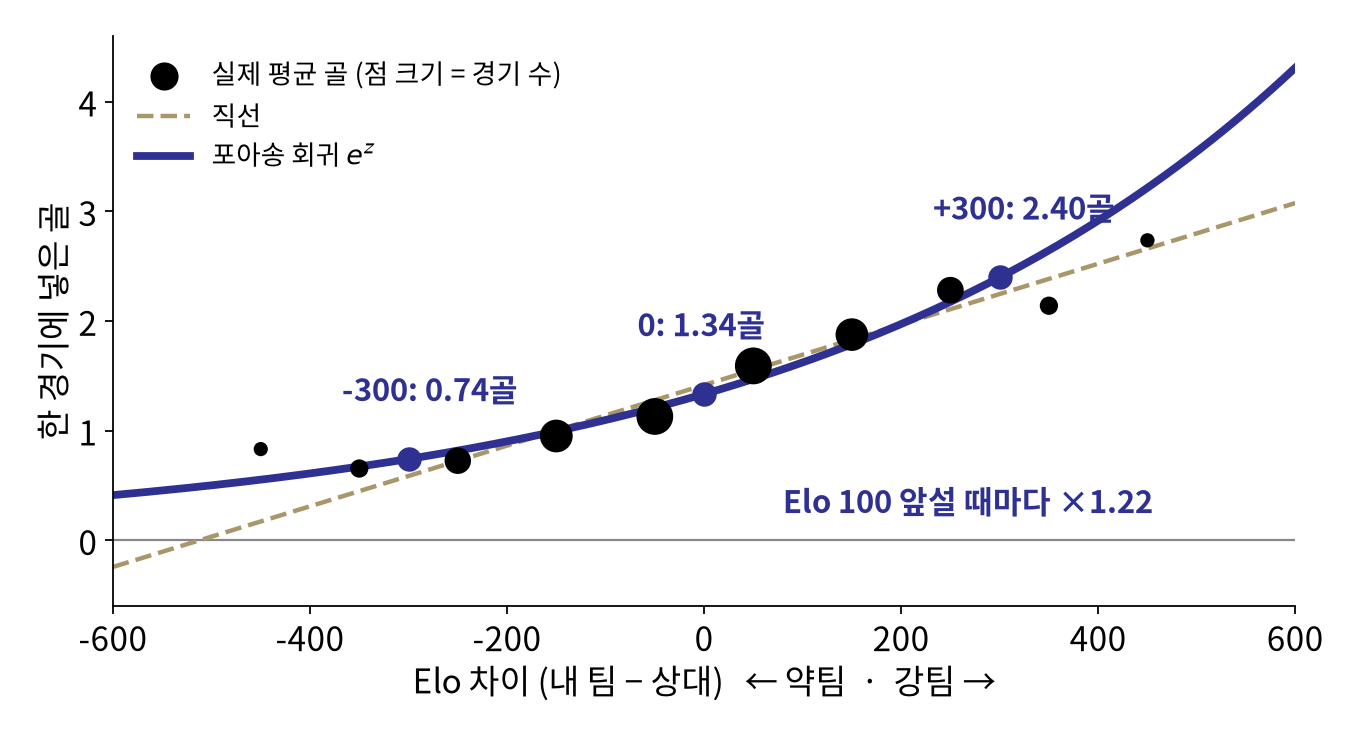
\includegraphics[width=0.58\linewidth]{glm_goals_pois.png}\par\vskip0.2em
{\large 골 $= e^{\,0.289 + 0.00195 \times \text{Elo 차이}}$ \quad $-300$: 0.74골 \;·\; 0: 1.34골 \;·\; $+300$: 2.40골}\\[0.2em]
{\large Elo 100 앞설 때마다 \kb{$\times 1.22$} ($e^{0.195}$) \quad 가장 약한 쪽 ($-575$) 도 \kb{0.43골} (직선은 $-0.17$)}
\vfill
\note{2136줄로 포아송 회귀를 학습하면 넣은 골은 e의 0.289 더하기 0.00195 곱하기 Elo 차이입니다. 실력이 같으면 1.34골, 300점 앞서면 2.40골, 300점 뒤지면 0.74골을 예측합니다. Elo가 100점 앞설 때마다 e의 0.195, 1.22배씩 늘어납니다. 그래서 더해 가는 직선이 아니라 곱해 가는 지수 곡선이고, 검은 점, 실제 평균을 직선보다 잘 따라갑니다. 직선이 음수를 예측했던 가장 약한 쪽, 575점 뒤진 경우도 0.43골로 양수입니다. 학습은 다음에 볼 같은 경사하강법으로 했고, sklearn의 PoissonRegressor와 같은 답이 나옵니다.}
\end{frame}

% --- 소프트맥스
\begin{frame}{클래스가 여럿이면: 소프트맥스}
\vfill
\centering
{\LARGE\[ P(y = k \mid x) = \frac{e^{\,z_k}}{\sum_{j=1}^{K} e^{\,z_j}} \qquad z_k = w_{k0} + w_{k1}\,x \]}\vskip0.5em
{\large 클래스마다 직선 하나 \;$\to$\; $e^{z}$ 로 양수 \;$\to$\; 합으로 나눠 \kb{더하면 1}}\\[0.5em]
{\large 클래스가 2개면: \;$\dfrac{e^{z_1}}{e^{z_1} + e^{z_0}} = \sigma(z_1 - z_0)$ \;=\; \kb{로지스틱회귀}}\\[0.4em]
{\small 범주형 분포 (categorical) 를 지수족 꼴로 쓰면 나오는 함수 \quad 유도는 CS229 노트 2.3절}
\vfill
\note{클래스가 셋 이상이면 범주형 분포를 씁니다. 이것도 지수족 꼴로 정리할 수 있고, 같은 요리법을 따라가면 소프트맥스라는 함수가 나옵니다. 유도는 길어서 결과만 봅시다. 클래스마다 직선 z k를 하나씩 둡니다. 각 z에 e를 씌워 양수로 만들고, 전부 더한 것으로 나눠서 합이 1이 되게 합니다. 그게 클래스 k의 확률입니다. 클래스가 두 개일 때 계산해 보면, e의 z1 나누기 e의 z1 더하기 e의 z0은 분자 분모를 e의 z1로 나누면 1 나누기 1 더하기 e의 마이너스 z1 빼기 z0, 시그모이드입니다. 소프트맥스는 로지스틱회귀를 클래스 여러 개로 넓힌 것입니다.}
\end{frame}

% --- 소프트맥스 결과
\begin{frame}{붓꽃 150송이: 꽃잎 길이 하나로 세 종}
\vfill
\centering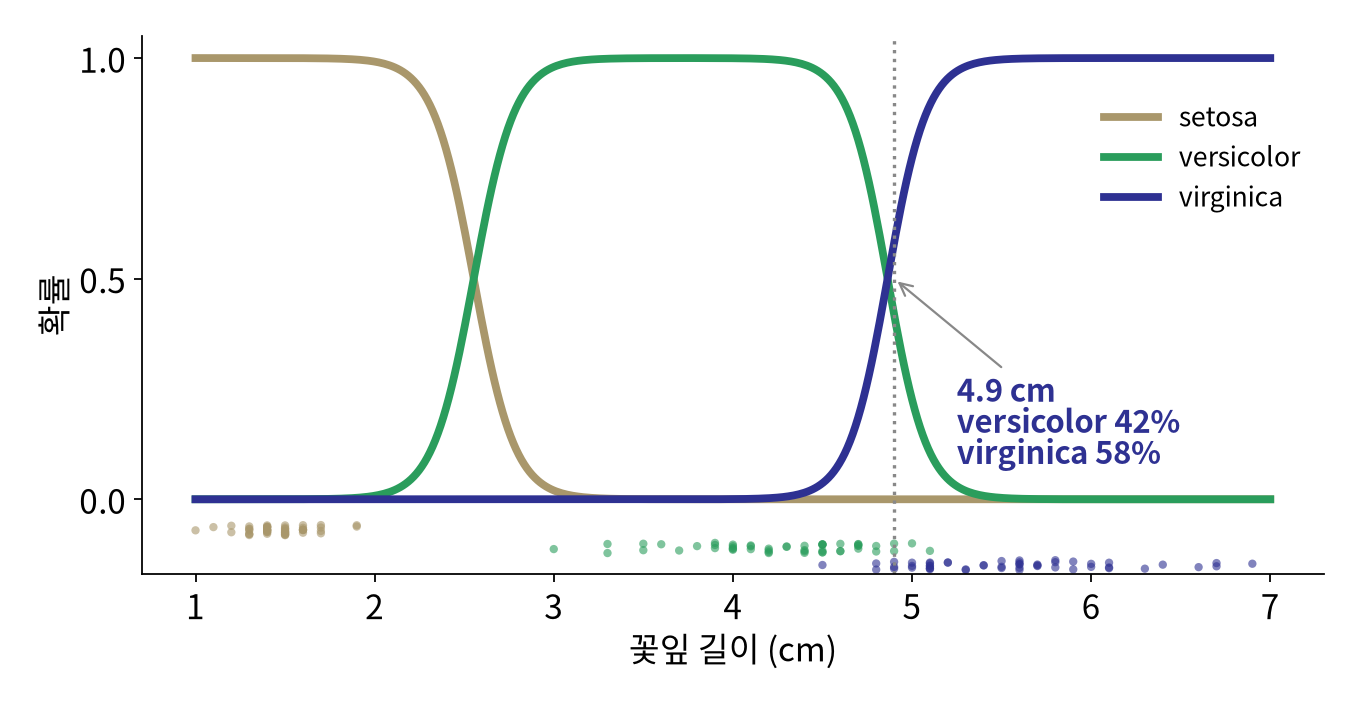
\includegraphics[width=0.58\linewidth]{glm_softmax.png}\par\vskip0.2em
{\large 꽃잎 4.9 cm: versicolor \kb{42\%} · virginica \kb{58\%} \quad 세 확률의 합은 언제나 1}\\[0.2em]
{\large 경계는 두 곳: 약 2.6 cm (setosa | versicolor) · 약 4.9 cm (versicolor | virginica)}
\vfill
\note{붓꽃 150송이로 꽃잎 길이 하나만 넣어 소프트맥스 회귀를 학습했습니다. 아래 점들이 실제 꽃이고, 세 곡선이 각 종일 확률입니다. 꽃잎이 짧으면 setosa, 중간이면 versicolor, 길면 virginica입니다. 어느 길이에서든 세 확률을 더하면 1입니다. 경계는 확률이 뒤바뀌는 곳, 약 2.6센티와 4.9센티 두 곳입니다. 4.9센티 꽃은 versicolor 42퍼센트, virginica 58퍼센트로 애매합니다. 실제로 4.5에서 5.1센티 사이는 두 종이 섞여 있습니다. 이 붓꽃 데이터는 다음 주 결정 트리에서도 다시 씁니다.}
\end{frame}

% --- 한 표
\begin{frame}{한 가족: 분포만 바꾸면 모델이 나온다}
\vfill
\centering
\renewcommand{\arraystretch}{1.7}
{\large\begin{tabular}{l|l|c|c|l}
$y$ & 분포 & 매개변수 $z$ & 예측 $\hat y = g(z)$ & 모델\\ \hline
실수 & 정규 & $\mu$ & $z$ & 선형회귀\\
0 / 1 & 베르누이 & $\log\frac{\phi}{1-\phi}$ & $\sigma(z)$ & 로지스틱회귀\\
개수 & 포아송 & $\log\lambda$ & $e^{z}$ & 포아송 회귀\\
$K$ 개 중 하나 & 범주형 & (벡터) & $\mathrm{softmax}(z)$ & 소프트맥스 회귀
\end{tabular}}\\[1.0em]
{\large 직선 $z$ 는 그대로 \;·\; 바깥 함수 $g$ 만 바뀐다}\\[0.3em]
{\small $g$ = response function, \;$g^{-1}$ = \kb{link function} (로지스틱: 로그 오즈, 포아송: $\log$)}
\vfill
\note{지금까지를 한 표로 모읍니다. y가 실수면 정규분포, z는 뮤, 예측은 z 그대로, 선형회귀입니다. 0과 1이면 베르누이, z는 로그 오즈, 예측은 시그모이드 z, 로지스틱회귀입니다. 개수면 포아송, z는 log 람다, 예측은 e의 z, 포아송 회귀입니다. 클래스가 여럿이면 범주형, 예측은 소프트맥스, 소프트맥스 회귀입니다. 모든 줄에서 직선 z는 똑같고, 바깥에 씌우는 함수 g만 바뀝니다. 이 g를 반응 함수, 거꾸로 평균을 z로 바꾸는 함수를 링크 함수라고 부릅니다. 로지스틱회귀의 링크 함수는 로그 오즈, 포아송 회귀의 링크 함수는 로그입니다.}
\end{frame}

\section{학습}
% --- 손실 = -log p
\begin{frame}{손실은 어디서 오나: $-\log p$}
\vfill
\centering
{\LARGE\[ \text{loss} = -\log p(y;z) = \underbrace{-\,z\,y + a(z)}_{\text{\normalsize 분포마다 이 두 항}} \;+\; \text{const} \]}\vskip0.4em
\renewcommand{\arraystretch}{1.45}
{\large\begin{tabular}{l|l}
정규 & $\tfrac12 (y - \hat y)^2$ \;=\; \kb{오차 제곱}\\
베르누이 & $-\big[\,y\log\hat y + (1-y)\log(1-\hat y)\,\big]$ \;=\; \kb{교차 엔트로피}\\
포아송 & $\hat y - y\log\hat y$
\end{tabular}}\\[0.6em]
{\small 최대 가능도: 데이터가 나올 확률을 가장 크게 $=$ $-\log$ 확률의 합을 가장 작게}
\vfill
\note{손실은 어디서 왔을까요? GLM에서는 손실을 정하는 것도 요리법의 일부입니다. 학습 데이터가 나올 확률을 가장 크게 하는 w를 찾습니다. 이걸 최대 가능도라고 합니다. 확률을 크게 하는 것은 마이너스 로그 확률을 작게 하는 것과 같으니, 손실은 마이너스 log p입니다. 지수족 꼴에 넣으면 마이너스 z y 더하기 a of z, 그리고 w와 상관없는 상수입니다. 정규분포에서 계산하면 2분의 1 y 빼기 와이햇의 제곱, 1주차의 오차 제곱입니다. 베르누이에서 계산하면 지난 시간의 교차 엔트로피입니다. 그러니까 선형회귀가 오차 제곱을, 로지스틱회귀가 교차 엔트로피를 쓰는 건 따로 고른 게 아니라, 분포를 고르면 같이 정해지는 짝입니다. 포아송이면 와이햇 빼기 y log 와이햇입니다.}
\end{frame}

% --- 기울기 유도
\begin{frame}{미분하면: $a'(z)$ 가 곧 평균}
\vfill
\centering
{\large\begin{align*}
\frac{\partial\,\text{loss}}{\partial z} &= -y + a'(z) && \text{loss} = -z y + a(z) + \text{const}\\[0.3em]
&= -y + \textcolor{ksared}{\hat y} && a'(z) = \text{평균} = \hat y\\[0.3em]
\frac{\partial\,\text{loss}}{\partial w_1} &= (\hat y - y)\,x && z = w_0 + w_1 x
\end{align*}}\vskip0.1em
\renewcommand{\arraystretch}{1.2}
{\large\begin{tabular}{l|c|c|c}
 & $a(z)$ & $a'(z)$ & 평균\\ \hline
베르누이 & $\log(1 + e^{z})$ & $\frac{e^{z}}{1 + e^{z}} = \sigma(z)$ & $\phi$ \;\checkmark\\
정규 & $\tfrac12z^2$ & $z$ & $\mu$ \;\checkmark\\
포아송 & $e^{z}$ & $e^{z}$ & $\lambda$ \;\checkmark
\end{tabular}}
\vfill
\note{이제 오늘의 질문에 답할 차례입니다. 손실 마이너스 z y 더하기 a of z를 z로 미분하면 마이너스 y 더하기 a 프라임 z입니다. 여기서 놀라운 사실이 있습니다. a 프라임 z가 언제나 그 분포의 평균입니다. 아래 표로 확인해 봅시다. 베르누이의 a는 log 1 더하기 e의 z, 미분하면 시그모이드 z, 평균 파이입니다. 정규분포의 a는 2분의 1 z제곱, 미분하면 z, 평균 뮤입니다. 포아송의 a는 e의 z, 미분해도 e의 z, 평균 람다입니다. 평균은 곧 예측 와이햇이니, z로 미분한 값은 와이햇 빼기 y입니다. 마지막으로 z가 w0 더하기 w1 x이니 연쇄 법칙으로 x를 곱하면, w1으로 미분한 값은 와이햇 빼기 y 곱하기 x입니다.}
\end{frame}

% --- 한 번 더 미분: a'' = 분산 → 볼록
\begin{frame}{한 번 더 미분하면: $a''(z)$ 는 분산 $\to$ 손실은 볼록}
\vfill
\centering
{\Large\[ \frac{\partial^2\,\text{loss}}{\partial z^2} = a''(z) = \text{Var}(y) \;\ge\; 0 \]}\vskip0.4em
\renewcommand{\arraystretch}{1.2}
{\large\begin{tabular}{l|c|c}
 & $a''(z)$ & 분산\\ \hline
베르누이 & $\sigma(z)\,\big(1 - \sigma(z)\big)$ & $\phi(1-\phi)$ \;\checkmark\\
정규 & $1$ & $\sigma^2 = 1$ \;\checkmark\\
포아송 & $e^{z}$ & $\lambda$ \;\checkmark
\end{tabular}}\\[0.5em]
{\large 기울기가 늘 0 이상 \;$\to$\; 손실은 \kb{그릇 모양} (볼록) \;$\to$\; 경사하강법이 \kb{하나뿐인 바닥}으로 간다}\\[0.3em]
{\small $z$ 가 $w$ 의 직선이라 $w$ 에 대해서도 볼록 \quad (CS229 강의 4)}
\vfill
\note{한 번 더 미분해 봅시다. 손실을 z로 두 번 미분하면 a 두 번 미분이고, 이건 언제나 y의 분산입니다. 표로 확인하면 베르누이는 시그모이드 곱하기 1 빼기 시그모이드, 파이 곱하기 1 빼기 파이로 베르누이의 분산입니다. 정규는 1, 시그마를 1로 두었으니 분산 1입니다. 포아송은 e의 z, 람다이고 포아송은 분산도 람다입니다. 분산은 음수가 될 수 없으니 두 번 미분한 값이 언제나 0 이상, 손실은 그릇 모양, 볼록 함수입니다. z가 w의 직선이니 w에 대해서도 볼록합니다. 그래서 GLM은 어느 분포를 고르든 바닥이 하나뿐이고, 경사하강법이 엉뚱한 곳에 갇히지 않습니다. 1주차 선형회귀와 지난 시간 로지스틱회귀의 손실이 그릇 모양이었던 이유입니다. 앤드류 응의 강의 4강에서 다루는 지수족의 성질입니다.}
\end{frame}

% --- 결과 크게
\begin{frame}{답: GLM 이면 기울기는 언제나 같은 모양}
\vfill
\centering
{\LARGE\[ \frac{\partial J}{\partial w_j} = \frac{1}{m}\sum_{i=1}^{m}\big(\,\hat y^{(i)} - y^{(i)}\,\big)\,x_j^{(i)} \]}\vskip0.6em
{\large 선형 \;·\; 로지스틱 \;·\; 포아송 \;·\; 소프트맥스 \;$\to$\; 경사하강법 코드는 \kb{예측 한 줄만} 다르다}\\[0.5em]
{\large \texttt{yhat = z} \;/\; \texttt{sigmoid(z)} \;/\; \texttt{exp(z)} \;/\; \texttt{softmax(z)}}\\[0.4em]
{\small 우연이 아니다: 분포와 손실이 짝 ($-\log p$) 이라서 $a'(z) =$ 평균이 맞물린다}
\vfill
\note{그래서 오늘의 질문의 답은 이렇습니다. GLM이면 기울기는 언제나 오차 와이햇 빼기 y 곱하기 입력의 평균입니다. 선형회귀, 로지스틱회귀, 포아송 회귀, 소프트맥스 회귀 모두 같습니다. 경사하강법 코드에서 예측하는 한 줄만, z 그대로, 시그모이드, exp, 소프트맥스로 바꾸면 됩니다. 오늘 월드컵 포아송 회귀도 로지스틱회귀 코드에서 시그모이드를 exp로 바꿔서 학습했습니다. 우연이 아니라, 분포를 고르면 손실이 마이너스 log p로 짝지어 정해지고, 그 미분에서 a 프라임이 평균이 되어 맞물리기 때문입니다.}
\end{frame}

\section{신경망}
% --- 신경망의 마지막 층
\begin{frame}{신경망으로 이어진다: 마지막 층이 GLM}
\vfill
\centering
\begin{tikzpicture}[node distance=1.1cm, every node/.style={font=\large},
  box/.style={draw, rounded corners=3pt, thick, minimum height=1.0cm, minimum width=1.6cm, align=center}]
\node[box] (x) {입력\\$x$};
\node[box, right=of x, fill=gray!10] (h) {숨은 층들\\특징 $h$};
\node[box, right=of h, draw=ksablue, fill=ksablue!8] (z) {$z = w \cdot h + b$};
\node[box, right=of z, draw=ksablue, fill=ksablue!8] (g) {$\hat y = g(z)$};
\node[box, right=of g] (L) {손실\\$-\log p$};
\draw[-{Stealth},thick] (x) -- (h); \draw[-{Stealth},thick] (h) -- (z); \draw[-{Stealth},thick] (z) -- (g); \draw[-{Stealth},thick] (g) -- (L);
\draw[ksablue, thick, dashed, rounded corners] ([xshift=-6pt,yshift=8pt]z.north west) rectangle ([xshift=6pt,yshift=-8pt]g.south east);
\node[ksablue, font=\large\bfseries, above=10pt of $(z.north)!0.5!(g.north)$] {마지막 층 $=$ GLM};
\draw[-{Stealth}, ultra thick, ksared] ([yshift=-14pt]L.south) to[bend left=18] node[below, font=\large\bfseries] {역전파의 시작: $\hat y - y$} ([yshift=-14pt]z.south);
\end{tikzpicture}\vskip1.0em
{\large 분류 신경망의 끝 $=$ 로지스틱 / 소프트맥스 회귀 \quad 회귀 신경망의 끝 $=$ 선형회귀}\\[0.3em]
{\large 앞 층들은 $x$ 대신 \kb{좋은 특징 $h$} 를 만드는 일을 한다}
\vfill
\note{GLM은 딥러닝으로 그대로 이어집니다. 신경망은 입력 x를 숨은 층들에 통과시켜 특징 h를 만들고, 마지막 층에서 z 이퀄 w 점곱 h 더하기 b를 계산한 뒤 함수 g를 씌웁니다. 이 마지막 층이 바로 오늘 본 GLM입니다. 분류하는 신경망의 끝은 로지스틱회귀나 소프트맥스 회귀이고, 숫자를 맞히는 신경망의 끝은 선형회귀입니다. 앞의 층들이 하는 일은 x 대신 GLM이 잘 쓸 수 있는 좋은 특징 h를 만드는 것입니다. 그리고 학습할 때 손실을 z로 미분한 값은, 오늘 본 대로 와이햇 빼기 y입니다. 역전파는 바로 이 와이햇 빼기 y에서 시작해서 앞 층으로 전해집니다. 7주차 역전파에서 다시 만납니다.}
\end{frame}

% --- 분포 하나에서 출력 함수와 손실이 둘 다
\begin{frame}{분포는 activation 도 loss 도 아니다: 둘 다 분포에서 나온다}
\vfill
\centering
\begin{tikzpicture}[every node/.style={font=\large},
  box/.style={draw, rounded corners=3pt, thick, minimum height=1.0cm, minimum width=3.4cm, align=center}]
\node[box, draw=ksablue, fill=ksablue!8, font=\Large\bfseries] (d) {분포 하나 고르기};
\node[box, below left=1.3cm and 0.6cm of d] (g) {출력 함수 $g(z)$\\{\normalsize 마지막 층의 activation}};
\node[box, below right=1.3cm and 0.6cm of d] (l) {손실 함수\\{\normalsize loss}};
\draw[-{Stealth}, thick] (d.south) -- node[left=6pt, font=\normalsize] {평균을 $z$ 로 풀기} (g.north);
\draw[-{Stealth}, thick] (d.south) -- node[right=6pt, font=\normalsize] {$-\log p$} (l.north);
\node[below=0.25cm of g, font=\normalsize] {예: 베르누이 $\to$ 시그모이드 $\sigma(z)$};
\node[below=0.25cm of l, font=\normalsize] {예: 베르누이 $\to$ 이진 교차 엔트로피};
\end{tikzpicture}\vskip1.2em
{\large 같은 분포에서 나왔으니 \kb{짝}으로 다닌다 \;$\to$\; 미분하면 $\hat y - y$}\\[0.3em]
{\small 숨은 층의 activation (ReLU 등) 은 분포와 상관없다}
\vfill
\note{자주 헷갈리는 질문이 있습니다. 정규분포, 베르누이 같은 분포는 activation 함수일까요, 손실 함수일까요? 둘 다 아닙니다. 분포는 y가 이렇게 나온다는 가정입니다. 그리고 이 가정 하나에서 둘이 다 나옵니다. 분포의 평균을 z로 풀면 출력 함수 g가 나오고, 이게 신경망 마지막 층의 activation입니다. 분포에 마이너스 log를 씌우면 손실 함수가 나옵니다. 베르누이를 고르면 출력은 시그모이드, 손실은 이진 교차 엔트로피입니다. 같은 분포에서 나왔으니 둘은 짝으로 다니고, 그래서 미분하면 와이햇 빼기 y로 깔끔합니다. 단, 숨은 층의 ReLU 같은 activation은 분포와 상관없습니다. 마지막 층만입니다. 다음 쪽에서 네 분포의 짝을 표로 봅니다.}
\end{frame}

% --- 짝 맞추기
\begin{frame}{출력 함수와 손실은 짝으로 쓴다}
\vfill
\centering
\renewcommand{\arraystretch}{1.6}
{\large\begin{tabular}{l|c|l|l}
$y$ & 출력 $g(z)$ & 손실 & PyTorch\\ \hline
실수 & 그대로 & 오차 제곱 & \texttt{MSELoss}\\
0 / 1 & $\sigma$ & 이진 교차 엔트로피 & \texttt{BCEWithLogitsLoss}\\
$K$ 개 중 하나 & softmax & 교차 엔트로피 & \texttt{CrossEntropyLoss}\\
개수 & $e^{z}$ & 포아송 & \texttt{PoissonNLLLoss}
\end{tabular}}\\[1.0em]
{\large 짝이 맞으면 기울기 $= \hat y - y$ \quad \kq{짝이 어긋나면} ($\sigma$ + 오차 제곱): $(\hat y - y)\,\hat y(1-\hat y)$}\\[0.3em]
{\small PyTorch 의 \texttt{WithLogits} · \texttt{CrossEntropyLoss} 는 $g$ 를 손실 안에서 씌운다 $\to$ 마지막 층은 $z$ 만 낸다}
\vfill
\note{그래서 신경망을 만들 때 출력 함수와 손실은 짝으로 고릅니다. y가 실수면 출력은 그대로, 손실은 오차 제곱, PyTorch의 MSELoss입니다. 0과 1이면 시그모이드와 이진 교차 엔트로피, BCEWithLogitsLoss입니다. 여러 클래스면 소프트맥스와 교차 엔트로피, CrossEntropyLoss입니다. 개수면 e의 z와 포아송 손실, PoissonNLLLoss입니다. 짝이 맞으면 기울기가 와이햇 빼기 y로 깔끔합니다. 지난 시간에 본 것처럼 시그모이드에 오차 제곱을 쓰면 시그모이드의 미분 와이햇 곱하기 1 빼기 와이햇이 더 곱해져서, 크게 틀렸는데도 와이햇이 0이나 1 근처면 기울기가 거의 0이 되어 학습이 멈춥니다. 참고로 PyTorch의 WithLogits와 CrossEntropyLoss는 시그모이드나 소프트맥스를 손실 안에서 씌우기 때문에, 신경망의 마지막 층은 z만 내보내면 됩니다.}
\end{frame}

% --- 짝이 어긋나면: 오차 제곱 vs 교차 엔트로피
\begin{frame}{짝이 어긋나면: $\sigma$ 에 오차 제곱 vs 교차 엔트로피}
\vfill
\centering
{\large $z = w \cdot x$, \quad $\hat y = \sigma(z)$, \quad $d\hat y/dz = \hat y(1-\hat y)$}\\[0.2em]
\begin{columns}[T]
\begin{column}{0.47\textwidth}
\centering
{\large\kq{오차 제곱} (Squared Error)}\\[0.3em]
$\displaystyle L = \tfrac12(\hat y - y)^2$\\[0.3em]
$\displaystyle \frac{dL}{d\hat y} = \hat y - y$\\[0.3em]
$\displaystyle \frac{dL}{dw} = (\hat y - y)\cdot\textcolor{ksared}{\hat y(1-\hat y)}\cdot x$\\[0.3em]
{\small $\hat y(1-\hat y)$ 가 \kq{남는다}}
\end{column}
\begin{column}{0.47\textwidth}
\centering
{\large\kb{교차 엔트로피} (Cross Entropy)}\\[0.3em]
$\displaystyle L = -\big[\,y\log\hat y + (1-y)\log(1-\hat y)\,\big]$\\[0.3em]
$\displaystyle \frac{dL}{d\hat y} = \frac{\hat y - y}{\textcolor{ksared}{\hat y(1-\hat y)}}$\\[0.3em]
$\displaystyle \frac{dL}{dw} = (\hat y - y)\cdot x$\\[0.3em]
{\small $\hat y(1-\hat y)$ 가 \kb{지워진다}}
\end{column}
\end{columns}\vskip0.4em
\renewcommand{\arraystretch}{1.15}
{\large\begin{tabular}{l|c}
\multicolumn{2}{l}{정답 $y = 1$ 인데 $\hat y = 0.01$ (크게 틀림) 일 때 기울기 $(dL/dw) / x$}\\ \hline
오차 제곱 & $(0.01 - 1) \times 0.01 \times 0.99 = -0.0098$\\
교차 엔트로피 & $0.01 - 1 = -0.99$ \quad ($100$ 배)
\end{tabular}}
\vfill
\note{짝이 어긋나면 어떻게 되는지 식으로 직접 봅시다. 출력은 시그모이드, z는 w 점곱 x이고, 시그모이드의 미분은 와이햇 곱하기 1 빼기 와이햇입니다. 왼쪽은 오차 제곱입니다. 2분의 1 와이햇 빼기 y의 제곱을 와이햇으로 미분하면 와이햇 빼기 y입니다. 연쇄 법칙으로 시그모이드 미분과 x를 곱하면, 와이햇 빼기 y 곱하기 와이햇 곱하기 1 빼기 와이햇 곱하기 x입니다. 시그모이드 미분이 그대로 남습니다. 오른쪽은 교차 엔트로피, 베르누이의 마이너스 log p입니다. 와이햇으로 미분하면 마이너스 y 나누기 와이햇 더하기 1 빼기 y 나누기 1 빼기 와이햇이고, 통분하면 와이햇 빼기 y 나누기 와이햇 곱하기 1 빼기 와이햇입니다. 분모에 시그모이드 미분이 생겨서, 연쇄 법칙으로 곱하면 정확히 지워지고 와이햇 빼기 y 곱하기 x만 남습니다. 숫자로 보면 차이가 큽니다. 정답이 1인데 와이햇이 0.01로 크게 틀렸을 때, 오차 제곱의 기울기는 마이너스 0.0098, 교차 엔트로피는 마이너스 0.99로 100배 차이입니다. 오차 제곱은 크게 틀렸는데도 거의 움직이지 않습니다. 그래서 출력 함수와 손실을 짝으로 씁니다.}
\end{frame}

\section{연습}
% --- 문제풀이
\begin{frame}{문제풀이}
\vfill
\begin{enumerate}
\item 베르누이에서 $\phi = 0.8$ 이면 $z$ 는? \; ($\log 4 \approx 1.39$)\vskip0.6em
\item 월드컵 모델 $\hat y = e^{\,0.289 + 0.00195\,x}$ ($x$ = Elo 차이). Elo 가 200 앞서면 골은 몇 배? \; ($e^{0.39} \approx 1.48$)\vskip0.6em
\item 클래스 2개 소프트맥스에서 $z_1 = 3$, $z_0 = 1$ 이면 $P(y = 1)$ 은? \; ($\sigma(2) \approx 0.88$)\vskip0.6em
\item 포아송 회귀에서 정답 $y = 5$, 예측 $\hat y = 3$, 입력 $x = 2$. 이 데이터 하나의 $\partial\,\text{loss} / \partial w_1$ 은?\vskip0.6em
\item 일주일 동안 가게에 온 손님 수를 예측하는 신경망. 마지막 층의 출력 함수와 손실은?
\end{enumerate}
\vfill
\note{1번 답. z는 로그 오즈, log 0.8 나누기 0.2, log 4, 약 1.39입니다. 2번 답. 200점 앞서면 z가 0.39 늘고, 골은 e의 0.39, 약 1.48배가 됩니다. 100점마다 1.22배를 두 번 곱한 것과 같습니다. 3번 답. 시그모이드 z1 빼기 z0, 시그모이드 2, 약 0.88입니다. 4번 답. 와이햇 빼기 y는 3 빼기 5, 마이너스 2, 여기에 x 2를 곱해서 마이너스 4입니다. 음수니까 w1을 키워서 예측을 늘리는 쪽으로 갑니다. 포아송이어도 로지스틱회귀와 같은 계산입니다. 5번 답. 손님 수는 개수이니 포아송, 출력 함수는 e의 z, 손실은 포아송 손실, PyTorch의 PoissonNLLLoss입니다.}
\end{frame}

\section{정리}
% --- 정리
\begin{frame}{정리}
\vfill
\centering\large\begin{tabular}{l}
GLM \quad 분포 하나 고르기 + 예측 $=$ 평균 + 매개변수 $=$ 직선 $z$\\[0.5em]
지수족 \quad $p(y;z) = b(y)\exp(z y - a(z))$ \;(정규 · 베르누이 · 포아송 · 범주형)\\[0.5em]
가족 \quad 정규 $\to z$ \;·\; 베르누이 $\to \sigma(z)$ \;·\; 포아송 $\to e^{z}$ \;·\; 범주형 $\to$ softmax\\[0.5em]
학습 \quad 손실 $= -\log p$, 기울기는 언제나 $(\hat y - y)\,x$ \;($a'(z) =$ 평균) \;·\; $a'' =$ 분산 $\ge 0$ $\to$ 볼록\\[0.5em]
신경망 \quad 마지막 층 $=$ GLM, 역전파는 $\hat y - y$ 에서 시작\\[0.5em]
월드컵 2136줄 \quad Elo 100 앞설 때마다 골 $\times 1.22$, 직선과 달리 음수 없음
\end{tabular}
\vfill
\note{정리합니다. GLM은 y의 분포 하나를 고르고, 예측을 그 분포의 평균으로, 분포의 매개변수를 직선 z로 두는 요리법입니다. 정규, 베르누이, 포아송, 범주형 분포는 모두 지수족 꼴로 쓸 수 있습니다. 분포에 따라 예측은 z 그대로, 시그모이드, e의 z, 소프트맥스가 되고, 각각 선형회귀, 로지스틱회귀, 포아송 회귀, 소프트맥스 회귀입니다. 손실은 마이너스 log p이고, a 프라임이 평균이라서 기울기는 언제나 와이햇 빼기 y 곱하기 x이고, a 두 번 미분이 분산이라 손실은 언제나 볼록합니다. 신경망의 마지막 층도 GLM이고, 역전파는 와이햇 빼기 y에서 시작합니다.}
\end{frame}

% --- 참고 문헌
\begin{frame}{참고 문헌}
\vfill
\small
\begin{itemize}
\item Ng, A., \& Ma, T. CS229 Lecture Notes, Chapter 3: Generalized Linear Models. Stanford. \paperlink{https://cs229.stanford.edu/main_notes.pdf}
\item Ng, A. (2018). Lecture 4: Perceptron \& Generalized Linear Model, CS229 Autumn 2018. \paperlink{https://www.youtube.com/watch?v=iZTeva0WSTQ}
\item McCullagh, P., \& Nelder, J. A. (1989). \textit{Generalized Linear Models} (2nd ed.). Chapman \& Hall.
\item Jürisoo, M. International football results from 1872 (국가대표 경기 결과, CC0). Elo 는 World Football Elo Ratings (eloratings.net) 방식으로 직접 계산. \paperlink{https://github.com/martj42/international_results}
\item Fisher, R. A. (1936). The use of multiple measurements in taxonomic problems. \textit{Annals of Eugenics}, 7(2).
\item lichess.org open database, 2013년 1월 (CC0). \paperlink{https://database.lichess.org}
\end{itemize}
\vfill
\note{오늘 내용은 스탠퍼드 CS229 강의 노트의 3부, 일반화 선형 모델을 바탕으로 했습니다. 앤드류 응의 2018년 강의 4강 영상에서 같은 내용을 볼 수 있습니다. 월드컵 데이터는 1872년부터의 국가대표 경기 결과 공개 데이터이고, Elo 점수는 그 경기 기록으로 직접 계산했습니다. 붓꽃은 피셔의 1936년 데이터, 체스는 lichess 공개 데이터베이스입니다.}
\end{frame}
\end{document}
